\documentclass{standalone}
\usepackage{tikz}
\usetikzlibrary{calc, angles}

\begin{document}
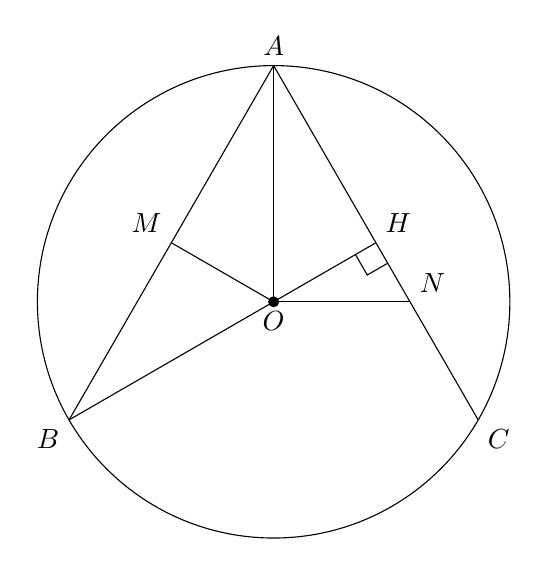
\begin{tikzpicture}
    % Define coordinates based on the visual structure
    \coordinate (O) at (0,0);
    \coordinate (A) at (90:3);
    \coordinate (B) at (210:3);
    \coordinate (C) at (330:3);
    
    % Draw the circle
    \draw (O) circle (3);
    
    % Draw chords AB and AC
    \draw (A) -- (B);
    \draw (A) -- (C);
    
    % Define M as midpoint of AB (implies OM perp AB)
    \coordinate (M) at ($(A)!0.5!(B)$);
    
    % Define N as intersection of AC and horizontal line through O to match visual
    \coordinate (N) at (intersection of A--C and O--{3,0});
    
    % Draw segments OA, OM, ON
    \draw (O) -- (A);
    \draw (O) -- (M);
    \draw (O) -- (N);
    
    % Instruction: From point B draw perpendicular to segment AC, mark foot H, draw BH, mark right angle
    
    % Calculate H as the projection of B onto AC
    \coordinate (H) at ($(A)!(B)!(C)$);
    
    % Draw segment BH
    \draw (B) -- (H);
    
    % Mark right angle at H
    \pic [draw, angle radius=3mm] {right angle = B--H--C};
    
    % Labels
    \node[above] at (A) {$A$};
    \node[below left] at (B) {$B$};
    \node[below right] at (C) {$C$};
    \node[above left] at (M) {$M$};
    \node[above right] at (N) {$N$};
    \node[below] at (O) {$O$};
    \node[above right] at (H) {$H$};
    
    % Draw center point O
    \fill (O) circle (2pt);
\end{tikzpicture}
\end{document}
